\documentclass[12pt]{article}
\usepackage[hmargin=1in,vmargin=1in]{geometry}
\usepackage{amsmath,amssymb}
\usepackage{graphicx}
\usepackage{comment}
\usepackage{mathtools}
\usepackage{listings}
\usepackage{float}
\usepackage{fixltx2e}

\usepackage{subcaption}
\usepackage{epstopdf}


%opening
\title{EE239AS - Project 4}
\author{Yuxin Jin (104195828), Jamie Lee (604589757),\\ David Hong (204588953) and Nick Cirillo (103834979)}

\begin{document}

\maketitle


\section{Popularity Prediction on Twitter}

With the increase in popularity of social media and communication, Twitter has emerged as a major platform for online networking which allows users to post and read 140-character messages called tweets. Tweets are publicly viewable via the website and users can subscribe to other user's tweets in the form "following" another user. A word, phrase or topic that is mentioned at a greater rate than others is said to be a "trending topic" and can often be recognized in the form of hashtags ie. \#TrendingTopic. These topics  become popular usually either through a specific event or topic that prompts people to discuss it or by purely users creating these discussions. This information easily allows users to obtain broad perspectives and recent updates. In addition to users, these trending and bursting topics have sparked recent interest in the scientific community to analyze and predict these topics.

In this project we seek to analyze such data by utilizing current and previous tweet activity for given hashtags in order to predict future tweet activity and behavior. Specifically we analyze tweet data for the 2015 Super Bowl (Seattle Seahawks vs. New England Patriots) from a period of two weeks before the game to a week after the game. We will use from related hashtags to train a regression model and use the same model to make predictions for other hashtags.


\subsection{Part 1:}

The training data was downloaded and statistics were calculated for each of the hashtags (\#gohawks, \#gopatriots, \#nfl, \#patriots, \#sb49 and \#superbowl). We report data on each hashtag for the total number of tweets, average number of tweets per hour, average number of retweets and average number of followers per users. Statistics for each hashtag can be found in the tables below.

\begin{table}[!h]
	\centering
	\begin{tabular}{| c | c | c | c |}
		\hline 
		Total \# of Tweets & 188135 \\\hline
		Avg. \# of Tweets per Hour & 276.669118 \\\hline
		Avg. \# of Retweets & 0.209164 \\\hline
		Avg \# of Followers of (77168) Users & 1720.634084 \\\hline
	\end{tabular} 
	\caption{\#gohawks statistics}
	\label{part1:tab1}
\end{table} 

\begin{table}[!h]
	\centering
	\begin{tabular}{| c | c | c | c |}
		\hline 
		Total \# of Tweets & 26231 \\\hline
		Avg. \# of Tweets per Hour & 58.551339 \\\hline
		Avg. \# of Retweets & 0.026838 \\\hline
		Avg \# of Followers of (18005) Users & 1559.278200 \\\hline
	\end{tabular} 
	\caption{\#gopatriots statistics}
	\label{part1:tab1}
\end{table} 

\begin{table}[!h]
	\centering
	\begin{tabular}{| c | c | c | c |}
		\hline 
		Total \# of Tweets & 259019 \\\hline
		Avg. \# of Tweets per Hour & 420.485390 \\\hline
		Avg. \# of Retweets & 0.050938 \\\hline
		Avg \# of Followers of (75167) Users & 4399.303205 \\\hline
	\end{tabular} 
	\caption{\#nfl statistics}
	\label{part1:tab1}
\end{table} 

\begin{table}[!h]
	\centering
	\begin{tabular}{| c | c | c | c |}
		\hline 
		Total \# of Tweets & 489710 \\\hline
		Avg. \# of Tweets per Hour & 736.406015 \\\hline
		Avg. \# of Retweets & 0.091462 \\\hline
		Avg \# of Followers of (326173) Users & 1865.903974 \\\hline
	\end{tabular} 
	\caption{\#patriots statistics}
	\label{part1:tab1}
\end{table} 

\begin{table}[!h]
	\centering
	\begin{tabular}{| c | c | c | c |}
		\hline 
		Total \# of Tweets & 826905 \\\hline
		Avg. \# of Tweets per Hour & 1531.305556 \\\hline
		Avg. \# of Retweets & 0.178023 \\\hline
		Avg \# of Followers of (590066) Users & 2247.285607 \\\hline
	\end{tabular} 
	\caption{\#sb49 statistics}
	\label{part1:tab1}
\end{table} 

\begin{table}[!h]
	\centering
	\begin{tabular}{| c | c | c | c |}
		\hline 
		Total \# of Tweets & 1348766 \\\hline
		Avg. \# of Tweets per Hour & 2207.472995 \\\hline
		Avg. \# of Retweets & 0.136686 \\\hline
		Avg \# of Followers of (689690) Users & 4228.627878 \\\hline
	\end{tabular} 
	\caption{\#superbowl statistics}
	\label{part1:tab1}
\end{table} 


The total tweet count per hour both both the \#SuperBowl and the \#NFL hashtags are also shown below. Both hashtags noticeably show initial trending prior to the SuperBowl, show significant bursting during the SuperBowl event and both die relatively quickly after the SuperBowl (Feburary 1, 2015).

\begin{figure}[H]
	\centering
	\begin{subfigure}{.45\textwidth}
		\centering
		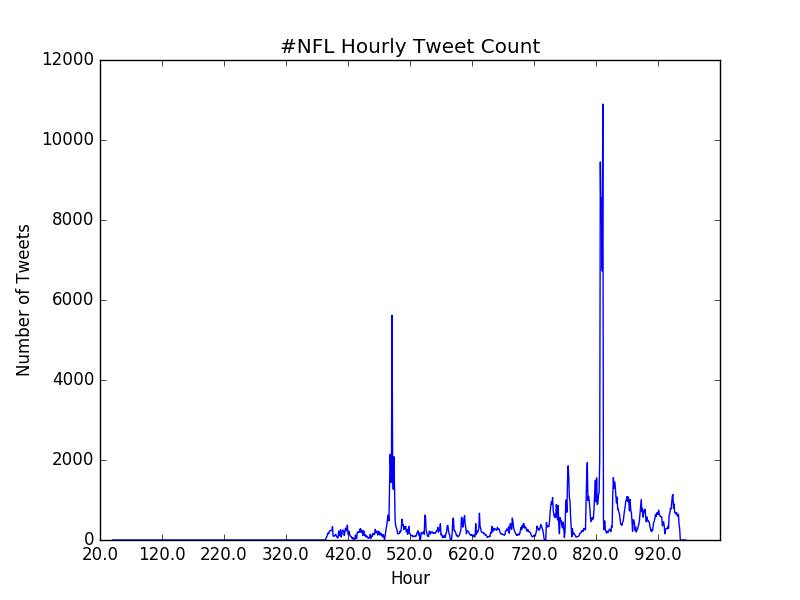
\includegraphics[width=\textwidth]{figures/1_NFL_histogram.jpeg}
		\centering
		\caption{\#NFL Hourly Tweet Count}
		\label{prob1:fig:1}
	\end{subfigure}%
	\hfill
	\begin{subfigure}{.45\textwidth}
		\centering
		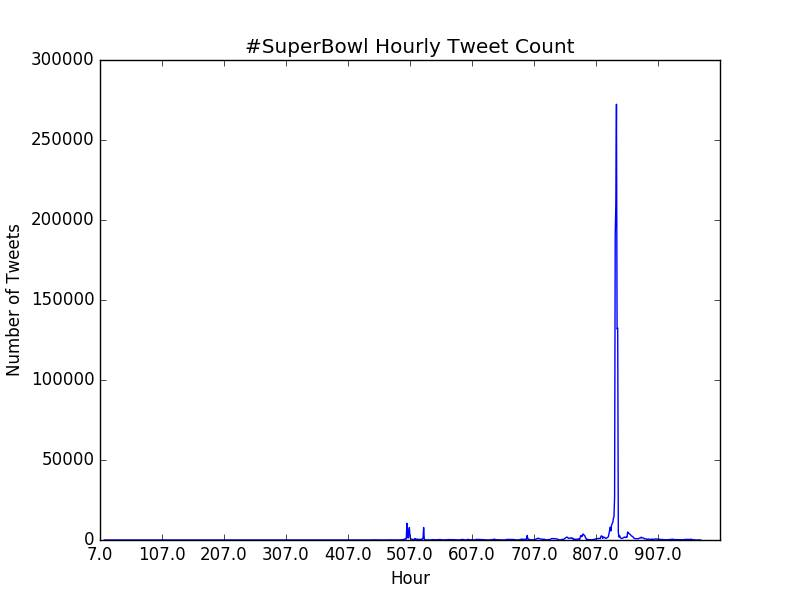
\includegraphics[width=\textwidth]{figures/1_SuperBowl_histogram.jpeg}
		\centering
		\caption{\#SuperBowl Hourly Tweet Count}
		\label{prob1:fig:2}
	\end{subfigure}
	\caption{Tweet counts per hour for tweet data obtained from 2 weeks prior to a week after the 2015 Superbowl}
\end{figure}

\subsection{Part 2:}

We now fit a linear regression model using 5 features to predict the numbers of tweets in a next hour using features extracted from a previous hour. The features used are: number of tweets, total number of retweets, sum of the number of followers of the users posting in the hashtag and the time of day.

The T-test feature values and P-value feature values are plotted below per hashtag. Additionally R\textsuperscript2 values are shown for 4 different linear methods per hashtag. The feature numbers correspond as follows. Feature 1: Total number of retweets, Feature 2:  sum of the number of followers of the users posting in the hashtag, Feature 3:  Maximum followers and Feature 4: Hour.

We used R\textsuperscript2 to explain our model's training accuracy. The best possible score is 1.0 however the value can be negative because it is possible the model can be arbitrarily worse. A constant model that always predicts the same value, disregarding the input features would achieve an R\textsuperscript2 of 0.0.

Different linear models were observed to have varying performance depending on the hashtag. For most of the hashtags the LARS Lasso method was observed to have the best possible score. Support Vector Regression was observed to have undesirable performance across all hashtags.

A t-test is a statistical examination of two population means. With relevance to our model the t-test represents how well that feature does with our model, the higher the t-test value the better.

The p-value represents a function of the observed results relative to our model and measures how extreme the observation is. Specifically, a small p-value indicates strong evidence against the null hypothesis and a large value indicates weak evidence against the null hypothesis.


%gohawks
\begin{table}[H]
	\centering
	\begin{tabular}{| c | c | c | c |}
		\hline 
		T-test Feature 1 & 32.254497 \\\hline
		T-test Feature 2 & 12339.208428 \\\hline
		T-test Feature 3 & 2.607192 \\\hline 
		T-test Feature 4 & nan \\\hline
		P-value Feature 1 & 0.185462 \\\hline
		P-value Feature 2 & 0.000000 \\\hline
		P-value Feature 3 & 0.182427 \\\hline
		P-value Feature 4 & nan \\\hline
	\end{tabular} 
	\caption{\#gohawks: T-test and P-value}
	\label{part1:tab1}
\end{table} 


\begin{table}[H]
	\centering
	\begin{tabular}{| c | c | c | c |}
		\hline 
		Linear Regression R\textsuperscript2  & -3.431273 \\\hline
		Logistic Regression R\textsuperscript2  & 0.137352 \\\hline
		Support Vector Regression R\textsuperscript2  & -0.083056 \\\hline
		LARS Lasso R\textsuperscript2  & 0.941716 \\\hline
	\end{tabular} 
	\caption{\#gohawks: R\textsuperscript2 Scores for different linear regression models}
	\label{part1:tab1}
\end{table} 

%gopatriots
\begin{table}[H]
	\centering
	\begin{tabular}{| c | c | c | c |}
		\hline 
		T-test Feature 1 & nan \\\hline
		T-test Feature 2 & 7148.513718 \\\hline
		T-test Feature 3 & 3.428438 \\\hline 
		T-test Feature 4 & nan \\\hline
		P-value Feature 1 & nan \\\hline
		P-value Feature 2 & 0.000000 \\\hline
		P-value Feature 3 & 0.181693 \\\hline
		P-value Feature 4 & nan \\\hline
	\end{tabular} 
	\caption{\#gopatriots: T-test and P-value}
	\label{part1:tab1}
\end{table} 


\begin{table}[H]
	\centering
	\begin{tabular}{| c | c | c | c |}
		\hline 
		Linear Regression R\textsuperscript2  & 0.866516 \\\hline
		Logistic Regression R\textsuperscript2  & 0.257283 \\\hline
		Support Vector Regression R\textsuperscript2  & -0.106411 \\\hline
		LARS Lasso R\textsuperscript2  & 0.857947 \\\hline
	\end{tabular} 
	\caption{\#gopatriots: R\textsuperscript2 Scores for different linear regression models}
	\label{part1:tab1}
\end{table} 

%nfl
\begin{table}[H]
	\centering
	\begin{tabular}{| c | c | c | c |}
		\hline 
		T-test Feature 1 & 75.215080 \\\hline
		T-test Feature 2 & 1604.618371 \\\hline
		T-test Feature 3 & 3.178866 \\\hline 
		T-test Feature 4 & nan \\\hline
		P-value Feature 1 & 0.432376 \\\hline
		P-value Feature 2 & 0.000003 \\\hline
		P-value Feature 3 & 0.202118 \\\hline
		P-value Feature 4 & nan \\\hline
	\end{tabular} 
	\caption{\#nfl: T-test and P-value}
	\label{part1:tab1}
\end{table} 


\begin{table}[H]
	\centering
	\begin{tabular}{| c | c | c | c |}
		\hline 
		Linear Regression R\textsuperscript2  & -2.498618 \\\hline
		Logistic Regression R\textsuperscript2  & 0.045448 \\\hline
		Support Vector Regression R\textsuperscript2  & -0.151815 \\\hline
		LARS Lasso R\textsuperscript2  & -2.148534 \\\hline
	\end{tabular} 
	\caption{\#nfl: R\textsuperscript2 Scores for different linear regression models}
	\label{part1:tab1}
\end{table} 

%patriots
\begin{table}[H]
	\centering
	\begin{tabular}{| c | c | c | c |}
		\hline 
		T-test Feature 1 & 61.083197 \\\hline
		T-test Feature 2 & 19299.952523 \\\hline
		T-test Feature 3 & 1.501174 \\\hline 
		T-test Feature 4 & nan \\\hline
		P-value Feature 1 & 0.226676 \\\hline
		P-value Feature 2 & 0.000000 \\\hline
		P-value Feature 3 & 0.388718 \\\hline
		P-value Feature 4 & nan \\\hline
	\end{tabular} 
	\caption{\#patriots: T-test and P-value}
	\label{part1:tab1}
\end{table} 


\begin{table}[H]
	\centering
	\begin{tabular}{| c | c | c | c |}
		\hline 
		Linear Regression R\textsuperscript2  & -2.291648 \\\hline
		Logistic Regression R\textsuperscript2  & 0.057163 \\\hline
		Support Vector Regression R\textsuperscript2  & -0.089487 \\\hline
		LARS Lasso R\textsuperscript2  & 0.912602 \\\hline
	\end{tabular} 
	\caption{\#patriots: R\textsuperscript2 Scores for different linear regression models}
	\label{part1:tab1}
\end{table} 

%sb49
\begin{table}[H]
	\centering
	\begin{tabular}{| c | c | c | c |}
		\hline 
		T-test Feature 1 & 243.116177 \\\hline
		T-test Feature 2 & 292994.277252 \\\hline
		T-test Feature 3 & 0.744969 \\\hline 
		T-test Feature 4 & nan \\\hline
		P-value Feature 1 & 0.289677 \\\hline
		P-value Feature 2 & 0.000000 \\\hline
		P-value Feature 3 & 0.472409 \\\hline
		P-value Feature 4 & nan \\\hline
	\end{tabular} 
	\caption{\#sb49: T-test and P-value}
	\label{part1:tab1}
\end{table} 


\begin{table}[H]
	\centering
	\begin{tabular}{| c | c | c | c |}
		\hline 
		Linear Regression R\textsuperscript2  & 0.941199 \\\hline
		Logistic Regression R\textsuperscript2  & 0.055304 \\\hline
		Support Vector Regression R\textsuperscript2  & -0.084825 \\\hline
		LARS Lasso R\textsuperscript2  & 0.949693 \\\hline
	\end{tabular} 
	\caption{\#sb49: R\textsuperscript2 Scores for different linear regression models}
	\label{part1:tab1}
\end{table} 

%superbowl
\begin{table}[H]
	\centering
	\begin{tabular}{| c | c | c | c |}
		\hline 
		T-test Feature 1 & 659.440411 \\\hline
		T-test Feature 2 & 30766.778560 \\\hline
		T-test Feature 3 & 0.908156 \\\hline 
		T-test Feature 4 & nan \\\hline
		P-value Feature 1 & 0.302070 \\\hline
		P-value Feature 2 & 0.000000 \\\hline
		P-value Feature 3 & 0.422320 \\\hline
		P-value Feature 4 & nan \\\hline
	\end{tabular} 
	\caption{\#superbowl: T-test and P-value}
	\label{part1:tab1}
\end{table} 


\begin{table}[H]
	\centering
	\begin{tabular}{| c | c | c | c |}
		\hline 
		Linear Regression R\textsuperscript2  & -0.102577 \\\hline
		Logistic Regression R\textsuperscript2  & 0.042759 \\\hline
		Support Vector Regression R\textsuperscript2  & -0.112585 \\\hline
		LARS Lasso R\textsuperscript2  & -0.098248 \\\hline
	\end{tabular} 
	\caption{\#superbowl: R\textsuperscript2 Scores for different linear regression models}
	\label{part1:tab1}
\end{table} 


\subsection{Part 3:}

In part 3 we design our own linear regression model using additional features at our discretion. In addition to the previous features used in Part 2. The features we added were the average number of tweets for each user, a threshold of the number of users who tweeted (threshold = 1), the number of users who tweeted greater than or equal to 3 times (threshold 3), the number of active users (users who tweet every hour in the past 6 hours) and the number of tweets with 100 characters or more (threshold = 100).

The T-test feature values and P-value feature values are plotted below per hashtag. Additionally R\textsuperscript2 values are shown for 4 different linear methods per hashtag. The feature numbers correspond as follows. Feature 1: Total number of retweets, Feature 2:  sum of the number of followers of the users posting in the hashtag, Feature 3:  Maximum followers, Feature 4: Hour, Feature 5: Average number of tweets for each user, Feature 6: Threshold of the number of users who tweeted (threshold 1), Feature 7: Threshold of the number of users who tweeted greater than or equal to 3 times (threshold 3) and Feature 8: the number of tweets with 100 characters or more (threshold = 100).

In our model we found the most significant features to be mainly: 1. The number of followers someone has, 2. The number of users tweeting that hashtag and to a lesser extent 3. the number of tweets that contain 100 characters or more. 

Scatter plots show the significance our top three features (showing the number of tweets vs  our feature) and all show linear relationships and therefore act as good predictors




%gohawks
\begin{table}[H]
	\centering
	\begin{tabular}{| c | c | c | c |}
		\hline 
		T-test Feature 1 & 32.254497 \\\hline
		T-test Feature 2 & 12339.208428 \\\hline
		T-test Feature 3 & 2.607192 \\\hline 
		T-test Feature 4 & nan \\\hline
		T-test Feature 5 & 2.305868 \\\hline
		T-test Feature 6 & 26540.184413 \\\hline
		T-test Feature 7 & 645.459722 \\\hline
		T-test Feature 8 & 1392.503026 \\\hline
		P-value Feature 1 & 0.185462 \\\hline
		P-value Feature 2 & 0.000000 \\\hline
		P-value Feature 3 & 0.182427 \\\hline
		P-value Feature 4 & nan \\\hline
		P-value Feature 5 & 0.451127 \\\hline
		P-value Feature 6 & 0.000000 \\\hline
		P-value Feature 7 & 0.000026 \\\hline
		P-value Feature 8 & 0.000000 \\\hline
	\end{tabular} 
	\caption{\#gohawks: T-test and P-value}
	\label{part1:tab1}
\end{table} 


\begin{table}[H]
	\centering
	\begin{tabular}{| c | c | c | c |}
		\hline 
		Linear Regression R\textsuperscript2  & 0.830944 \\\hline
		Logistic Regression R\textsuperscript2  & 0.137352 \\\hline
		Support Vector Regression R\textsuperscript2  & -0.083049 \\\hline
		LARS Lasso R\textsuperscript2  & 0.978351 \\\hline
	\end{tabular} 
	\caption{\#gohawks: R\textsuperscript2 Scores for different linear regression models}
	\label{part1:tab1}
\end{table} 


%gopatriots
\begin{table}[H]
	\centering
	\begin{tabular}{| c | c | c | c |}
		\hline 
		T-test Feature 1 & nan \\\hline
		T-test Feature 2 & 7148.513718 \\\hline
		T-test Feature 3 & 3.428438 \\\hline 
		T-test Feature 4 & nan \\\hline
		T-test Feature 5 & 22.746685 \\\hline
		T-test Feature 6 & 621064.374186 \\\hline
		T-test Feature 7 & nan \\\hline
		T-test Feature 8 & 7142.937408 \\\hline
		P-value Feature 1 & nan \\\hline
		P-value Feature 2 & 0.000000 \\\hline
		P-value Feature 3 & 0.181693 \\\hline
		P-value Feature 4 & nan \\\hline
		P-value Feature 5 & 0.572824 \\\hline
		P-value Feature 6 & 0.000000 \\\hline
		P-value Feature 7 & nan \\\hline
		P-value Feature 8 & 0.000000 \\\hline
	\end{tabular} 
	\caption{\#gopatriots: T-test and P-value}
	\label{part1:tab1}
\end{table} 


\begin{table}[H]
	\centering
	\begin{tabular}{| c | c | c | c |}
		\hline 
		Linear Regression R\textsuperscript2  & 0.989521 \\\hline
		Logistic Regression R\textsuperscript2  & 0.257283 \\\hline
		Support Vector Regression R\textsuperscript2  & -0.106411 \\\hline
		LARS Lasso R\textsuperscript2  & 0.916684 \\\hline
	\end{tabular} 
	\caption{\#gopatriots: R\textsuperscript2 Scores for different linear regression models}
	\label{part1:tab1}
\end{table} 


%nfl
\begin{table}[H]
	\centering
	\begin{tabular}{| c | c | c | c |}
		\hline 
		T-test Feature 1 & 75.215080 \\\hline
		T-test Feature 2 & 1604.618371 \\\hline
		T-test Feature 3 & 3.178866 \\\hline 
		T-test Feature 4 & nan \\\hline
		T-test Feature 5 & 6.831252 \\\hline
		T-test Feature 6 & 2187.079982 \\\hline
		T-test Feature 7 & 267.385951 \\\hline
		T-test Feature 8 & 1835.564400 \\\hline
		P-value Feature 1 & 0.432376 \\\hline
		P-value Feature 2 & 0.000003 \\\hline
		P-value Feature 3 & 0.202118 \\\hline
		P-value Feature 4 & nan \\\hline
		P-value Feature 5 & 0.183349 \\\hline
		P-value Feature 6 & 0.000000 \\\hline
		P-value Feature 7 & 0.000000 \\\hline
		P-value Feature 8 & 0.000000 \\\hline
	\end{tabular} 
	\caption{\#nfl: T-test and P-value}
	\label{part1:tab1}
\end{table} 


\begin{table}[H]
	\centering
	\begin{tabular}{| c | c | c | c |}
		\hline 
		Linear Regression R\textsuperscript2  & 0.978169 \\\hline
		Logistic Regression R\textsuperscript2  & 0.045448 \\\hline
		Support Vector Regression R\textsuperscript2  & -0.151815 \\\hline
		LARS Lasso R\textsuperscript2  & 0.991687 \\\hline
	\end{tabular} 
	\caption{\#nfl: R\textsuperscript2 Scores for different linear regression models}
	\label{part1:tab1}
\end{table} 


%patriots
\begin{table}[H]
	\centering
	\begin{tabular}{| c | c | c | c |}
		\hline 
		T-test Feature 1 & 61.083197 \\\hline
		T-test Feature 2 & 19299.952523 \\\hline
		T-test Feature 3 & 1.501174 \\\hline 
		T-test Feature 4 & nan \\\hline
		T-test Feature 5 & 0.425384 \\\hline
		T-test Feature 6 & 196192.985044 \\\hline
		T-test Feature 7 & 4203.146057 \\\hline
		T-test Feature 8 & 3147.501792 \\\hline
		P-value Feature 1 & 0.226676 \\\hline
		P-value Feature 2 & 0.000000 \\\hline
		P-value Feature 3 & 0.388718 \\\hline
		P-value Feature 4 & nan \\\hline
		P-value Feature 5 & 0.633074 \\\hline
		P-value Feature 6 & 0.000000 \\\hline
		P-value Feature 7 & 0.003434 \\\hline
		P-value Feature 8 & 0.000000 \\\hline
	\end{tabular} 
	\caption{\#patriots: T-test and P-value}
	\label{part1:tab1}
\end{table} 


\begin{table}[H]
	\centering
	\begin{tabular}{| c | c | c | c |}
		\hline 
		Linear Regression R\textsuperscript2  & 0.541453 \\\hline
		Logistic Regression R\textsuperscript2  & 0.057163 \\\hline
		Support Vector Regression R\textsuperscript2  & -0.089484 \\\hline
		LARS Lasso R\textsuperscript2  & 0.990319 \\\hline
	\end{tabular} 
	\caption{\#patriots: R\textsuperscript2 Scores for different linear regression models}
	\label{part1:tab1}
\end{table} 


%sb49
\begin{table}[H]
	\centering
	\begin{tabular}{| c | c | c | c |}
		\hline 
		T-test Feature 1 & 243.116177 \\\hline
		T-test Feature 2 & 292994.277252 \\\hline
		T-test Feature 3 & 0.744969 \\\hline 
		T-test Feature 4 & nan \\\hline
		T-test Feature 5 & 3.109246 \\\hline
		T-test Feature 6 & 1401642.010906 \\\hline
		T-test Feature 7 & 32016.027715 \\\hline
		T-test Feature 8 & 8617.255121 \\\hline
		P-value Feature 1 & 0.289677 \\\hline
		P-value Feature 2 & 0.000000 \\\hline
		P-value Feature 3 & 0.472409 \\\hline
		P-value Feature 4 & nan \\\hline
		P-value Feature 5 & 0.447412 \\\hline
		P-value Feature 6 & 0.000000 \\\hline
		P-value Feature 7 & 0.000000 \\\hline
		P-value Feature 8 & 0.000000 \\\hline
	\end{tabular} 
	\caption{\#sb49: T-test and P-value}
	\label{part1:tab1}
\end{table} 


\begin{table}[H]
	\centering
	\begin{tabular}{| c | c | c | c |}
		\hline 
		Linear Regression R\textsuperscript2  & 0.996203 \\\hline
		Logistic Regression R\textsuperscript2  & 0.055304 \\\hline
		Support Vector Regression R\textsuperscript2  & -0.084825 \\\hline
		LARS Lasso R\textsuperscript2  & 0.997678 \\\hline
	\end{tabular} 
	\caption{\#sb49: R\textsuperscript2 Scores for different linear regression models}
	\label{part1:tab1}
\end{table} 


%superbowl
\begin{table}[H]
	\centering
	\begin{tabular}{| c | c | c | c |}
		\hline 
		T-test Feature 1 & 659.440411 \\\hline
		T-test Feature 2 & 30766.778560 \\\hline
		T-test Feature 3 & 0.908156 \\\hline 
		T-test Feature 4 & nan \\\hline
		T-test Feature 5 & 4.231599 \\\hline
		T-test Feature 6 & 169100.241200 \\\hline
		T-test Feature 7 & 22053.868096 \\\hline
		T-test Feature 8 & 9162.252714 \\\hline
		P-value Feature 1 & 0.302070 \\\hline
		P-value Feature 2 & 0.000000 \\\hline
		P-value Feature 3 & 0.422320 \\\hline
		P-value Feature 4 & nan \\\hline
		P-value Feature 5 & 0.379419 \\\hline
		P-value Feature 6 & 0.000000 \\\hline
		P-value Feature 7 & 0.000000 \\\hline
		P-value Feature 8 & 0.000000 \\\hline
	\end{tabular} 
	\caption{\#superbowl: T-test and P-value}
	\label{part1:tab1}
\end{table} 


\begin{table}[H]
	\centering
	\begin{tabular}{| c | c | c | c |}
		\hline 
		Linear Regression R\textsuperscript2  & 0.996959 \\\hline
		Logistic Regression R\textsuperscript2  & 0.042759 \\\hline
		Support Vector Regression R\textsuperscript2  & -0.112585 \\\hline
		LARS Lasso R\textsuperscript2  & 0.997060 \\\hline
	\end{tabular} 
	\caption{\#superbowl: R\textsuperscript2 Scores for different linear regression models}
	\label{part1:tab1}
\end{table} 


%gohawks
\begin{figure}[H]
\centering
\begin{subfigure}{.45\textwidth}
  \centering
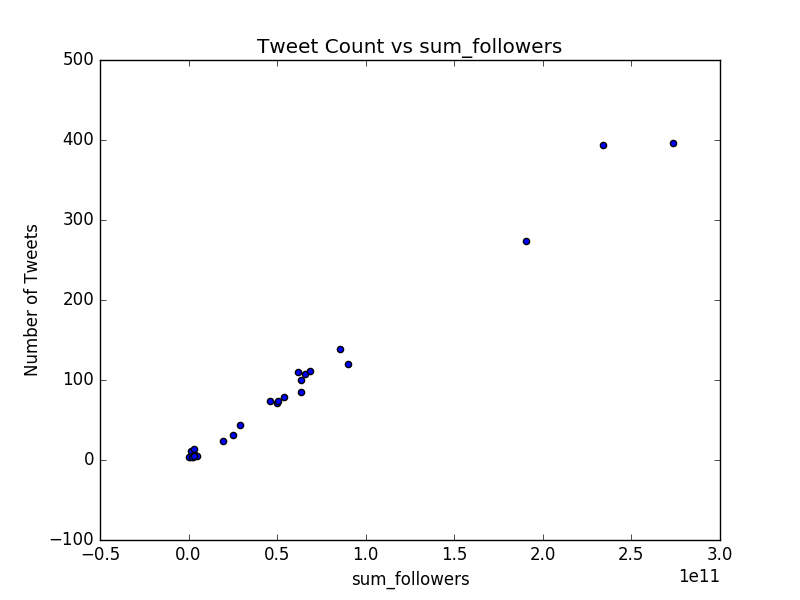
\includegraphics[width=\textwidth]{figures/count_vs_sum_tweets_gohawks.png}
\caption{Tweet Count vs Sum of Total Number of Followers}
\label{part1:fig:LC}
\end{subfigure}%
\hfill
\begin{subfigure}{.45\textwidth}
  \centering
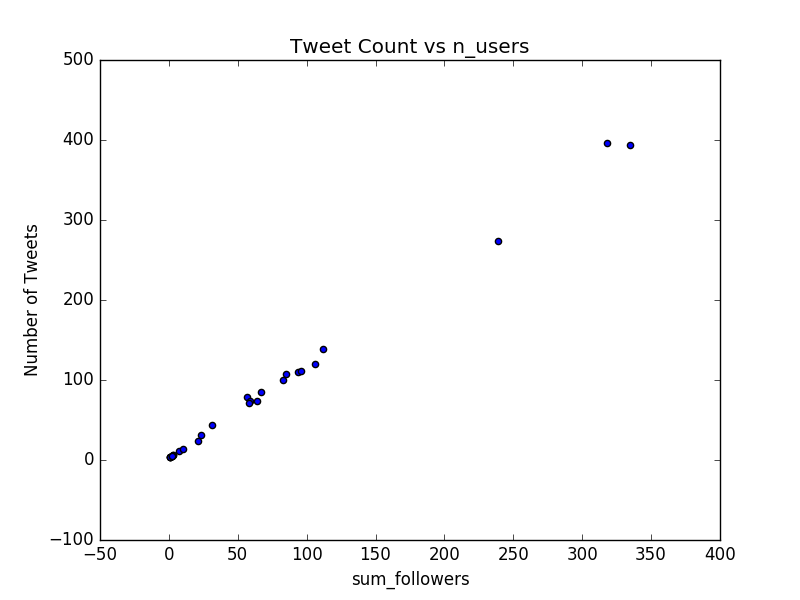
\includegraphics[width=\textwidth]{figures/count_vs_n_users_tweets_gohawks.png}
\caption{Tweet Count vs Number of Users Who Tweeted 3 or More Times Per Hour}
\label{part1:fig:LC}
\end{subfigure}

\begin{subfigure}{.45\textwidth}
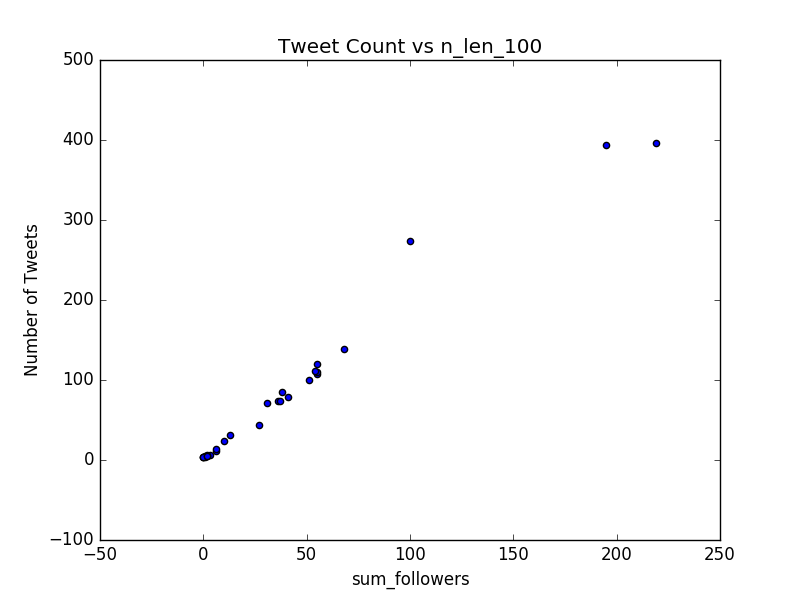
\includegraphics[width=\textwidth]{figures/count_vs_n_len_100_tweets_gohawks.png}
\caption{Tweet Count vs Number of Tweets with 100 or More Characters }
\label{part1:fig:LC}
\end{subfigure}

\caption{\#gohawks: Scatter plots for top 3 features in measurements}
\label{part1:fig}
\end{figure}

%gohawks
\begin{figure}[H]
\centering
\begin{subfigure}{.45\textwidth}
  \centering
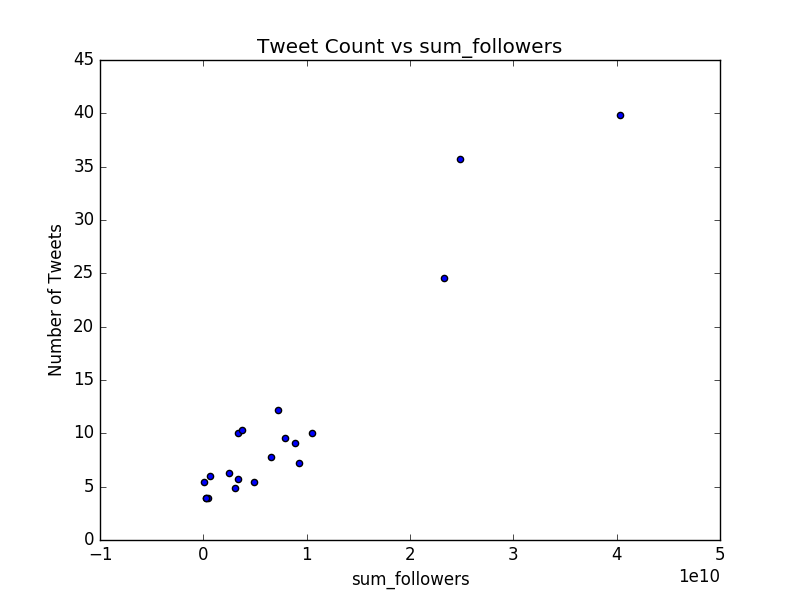
\includegraphics[width=\textwidth]{figures/count_vs_sum_tweets_gopatriots.png}
\caption{Tweet Count vs Sum of Total Number of Followers}
\label{part1:fig:LC}
\end{subfigure}%
\hfill
\begin{subfigure}{.45\textwidth}
  \centering
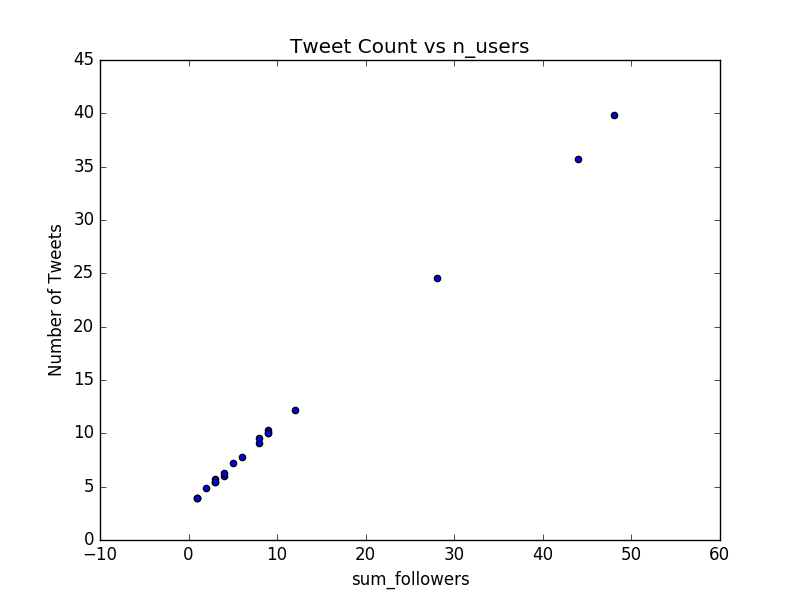
\includegraphics[width=\textwidth]{figures/count_vs_n_users_tweets_gopatriots.png}
\caption{Tweet Count vs Number of Users Who Tweeted 3 or More Times Per Hour}
\label{part1:fig:LC}
\end{subfigure}

\begin{subfigure}{.45\textwidth}
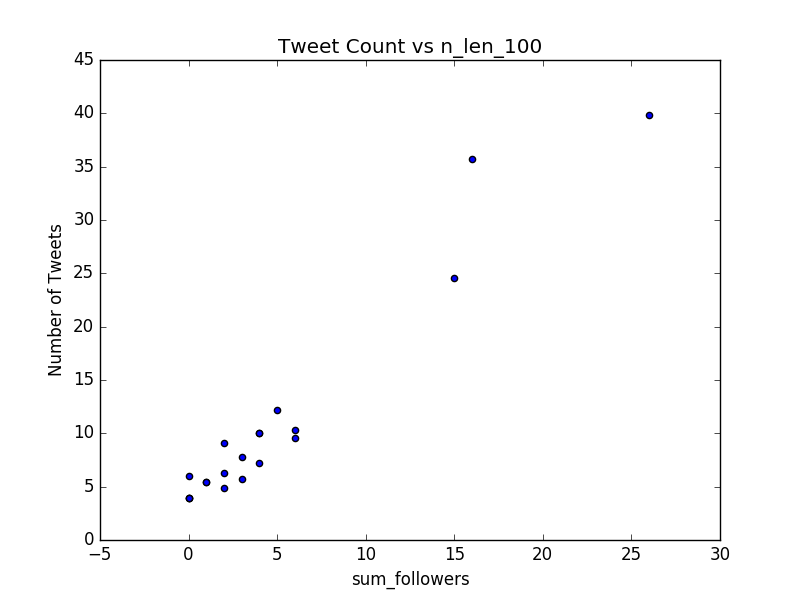
\includegraphics[width=\textwidth]{figures/count_vs_n_len_100_tweets_gopatriots.png}
\caption{Tweet Count vs Number of Tweets with 100 or More Characters }
\label{part1:fig:LC}
\end{subfigure}

\caption{\#gopatriots: Scatter plots for top 3 features in measurements}
\label{part1:fig}
\end{figure}


%nfl
\begin{figure}[H]
\centering
\begin{subfigure}{.45\textwidth}
  \centering
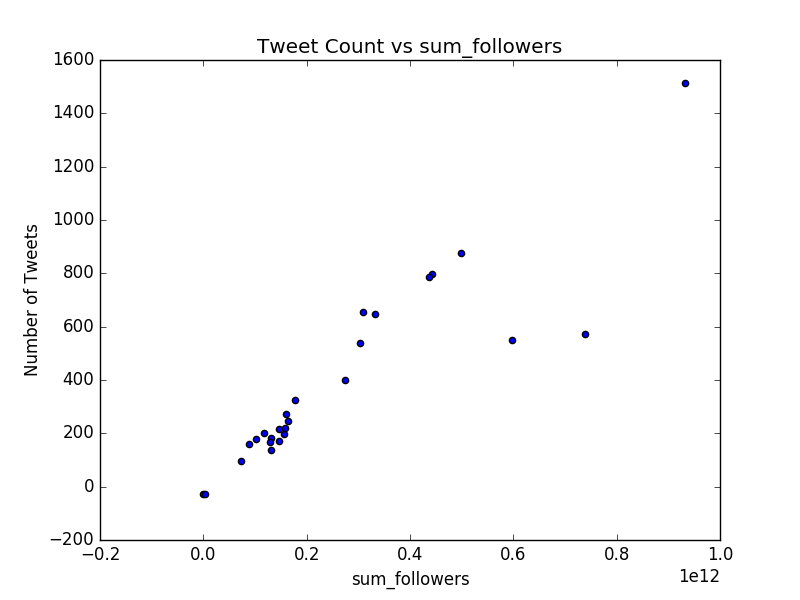
\includegraphics[width=\textwidth]{figures/count_vs_sum_tweets_nfl.png}
\caption{Tweet Count vs Sum of Total Number of Followers}
\label{part1:fig:LC}
\end{subfigure}%
\hfill
\begin{subfigure}{.45\textwidth}
  \centering
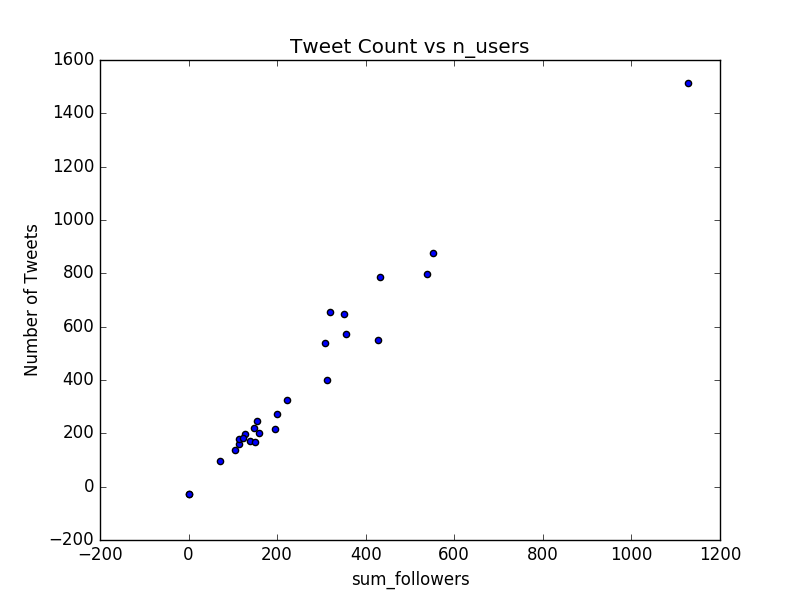
\includegraphics[width=\textwidth]{figures/count_vs_n_users_tweets_nfl.png}
\caption{Tweet Count vs Number of Users Who Tweeted 3 or More Times Per Hour}
\label{part1:fig:LC}
\end{subfigure}

\begin{subfigure}{.45\textwidth}
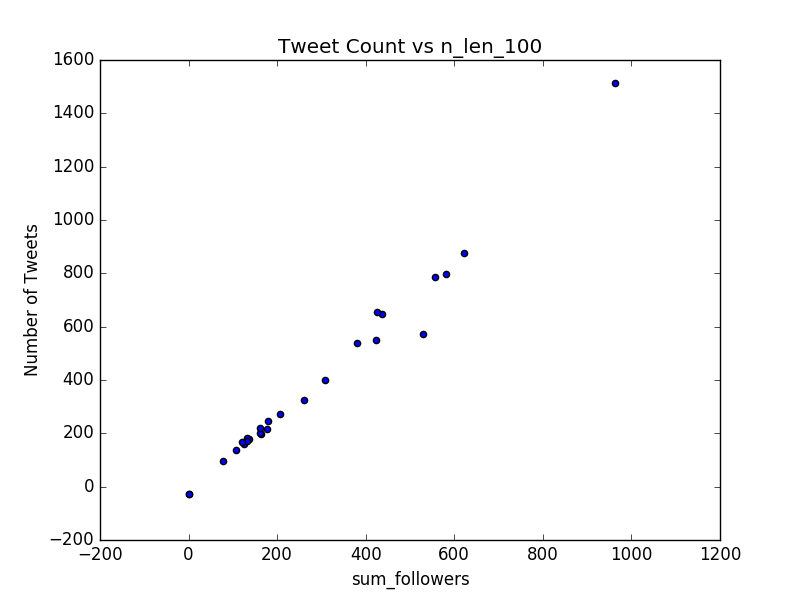
\includegraphics[width=\textwidth]{figures/count_vs_n_len_100_tweets_nfl.png}
\caption{Tweet Count vs Number of Tweets with 100 or More Characters }
\label{part1:fig:LC}
\end{subfigure}

\caption{\#nfl: Scatter plots for top 3 features in measurements}
\label{part1:fig}
\end{figure}


%patriots
\begin{figure}[H]
\centering
\begin{subfigure}{.45\textwidth}
  \centering
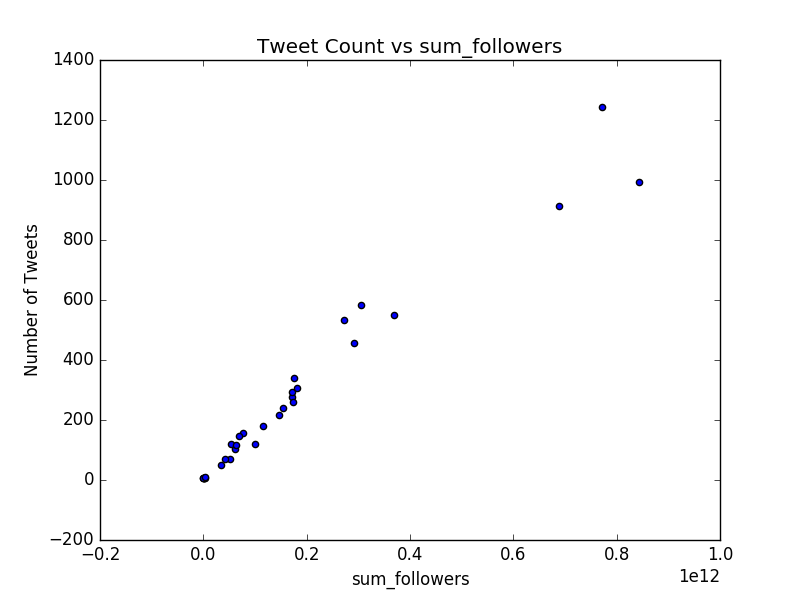
\includegraphics[width=\textwidth]{figures/count_vs_sum_tweets_patriots.png}
\caption{Tweet Count vs Sum of Total Number of Followers}
\label{part1:fig:LC}
\end{subfigure}%
\hfill
\begin{subfigure}{.45\textwidth}
  \centering
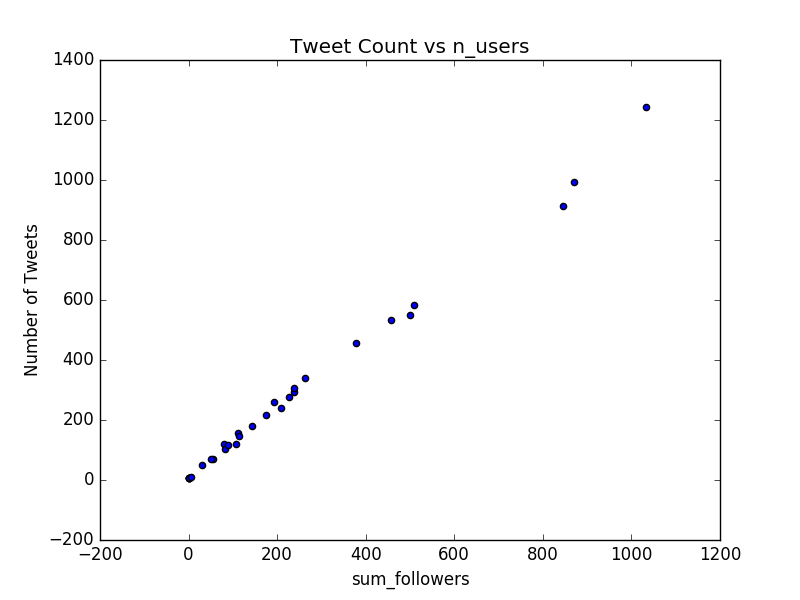
\includegraphics[width=\textwidth]{figures/count_vs_n_users_tweets_patriots.png}
\caption{Tweet Count vs Number of Users Who Tweeted 3 or More Times Per Hour}
\label{part1:fig:LC}
\end{subfigure}

\begin{subfigure}{.45\textwidth}
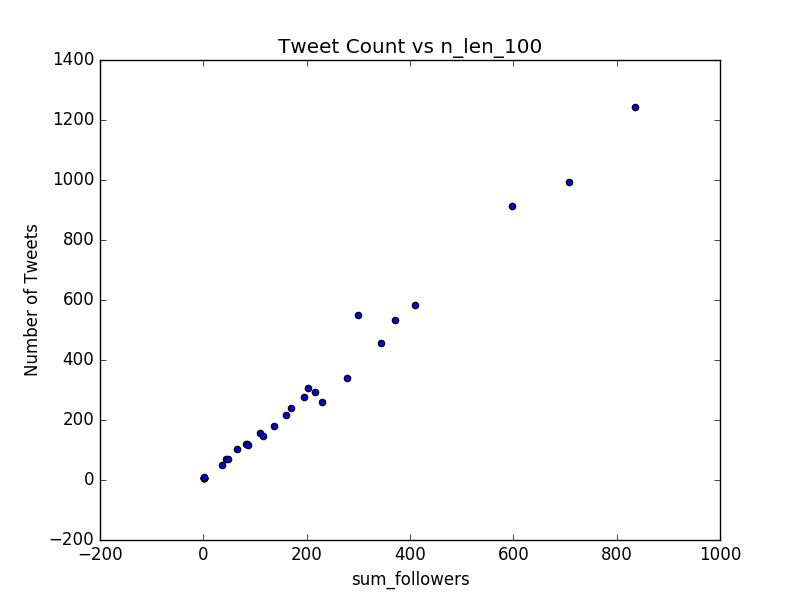
\includegraphics[width=\textwidth]{figures/count_vs_n_len_100_tweets_patriots.png}
\caption{Tweet Count vs Number of Tweets with 100 or More Characters }
\label{part1:fig:LC}
\end{subfigure}

\caption{\#patriots: Scatter plots for top 3 features in measurements}
\label{part1:fig}
\end{figure}


%sb49
\begin{figure}[H]
\centering
\begin{subfigure}{.45\textwidth}
  \centering
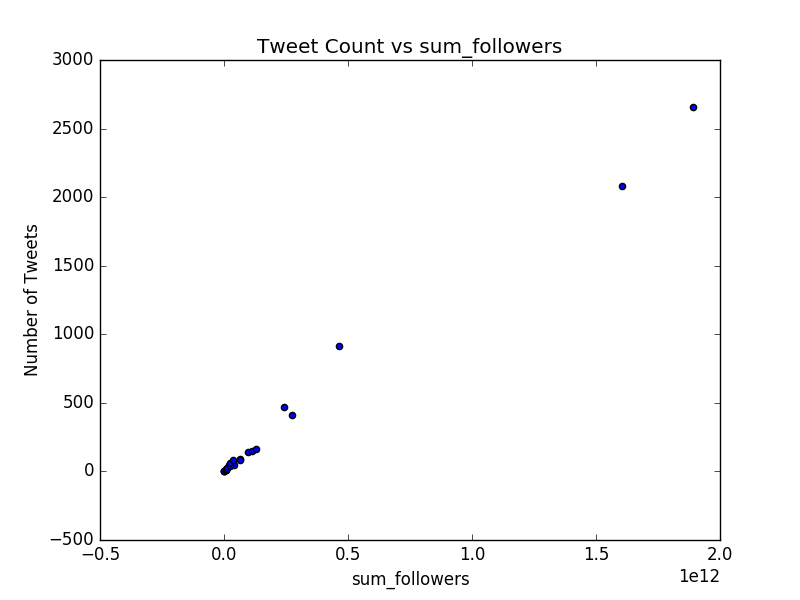
\includegraphics[width=\textwidth]{figures/count_vs_sum_tweets_sb49.png}
\caption{Tweet Count vs Sum of Total Number of Followers}
\label{part1:fig:LC}
\end{subfigure}%
\hfill
\begin{subfigure}{.45\textwidth}
  \centering
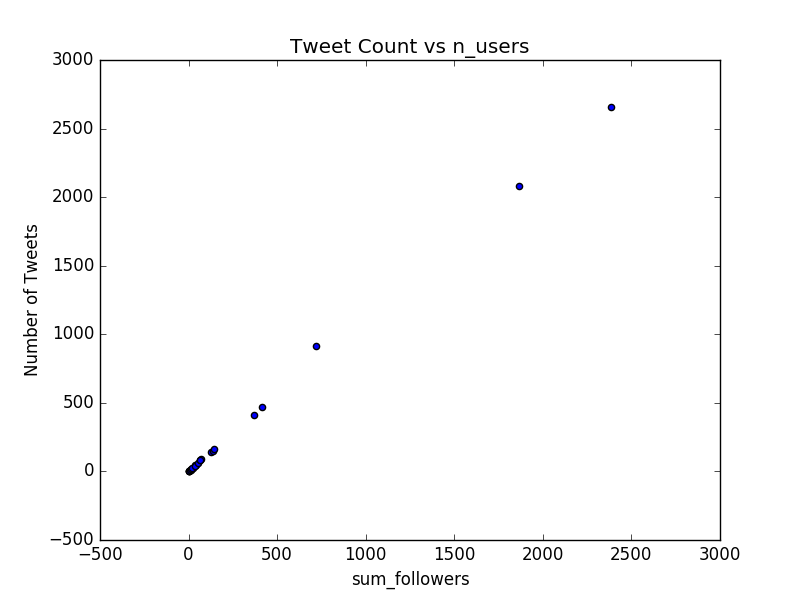
\includegraphics[width=\textwidth]{figures/count_vs_n_users_tweets_sb49.png}
\caption{Tweet Count vs Number of Users Who Tweeted 3 or More Times Per Hour}
\label{part1:fig:LC}
\end{subfigure}

\begin{subfigure}{.45\textwidth}
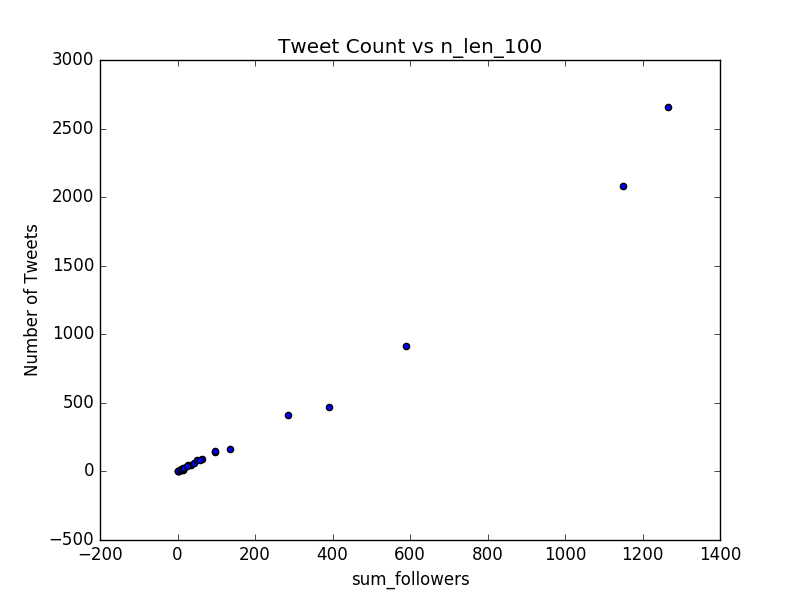
\includegraphics[width=\textwidth]{figures/count_vs_n_len_100_tweets_sb49.png}
\caption{Tweet Count vs Number of Tweets with 100 or More Characters }
\label{part1:fig:LC}
\end{subfigure}

\caption{\#sb49: Scatter plots for top 3 features in measurements}
\label{part1:fig}
\end{figure}

%superbowl
\begin{figure}[H]
\centering
\begin{subfigure}{.45\textwidth}
  \centering
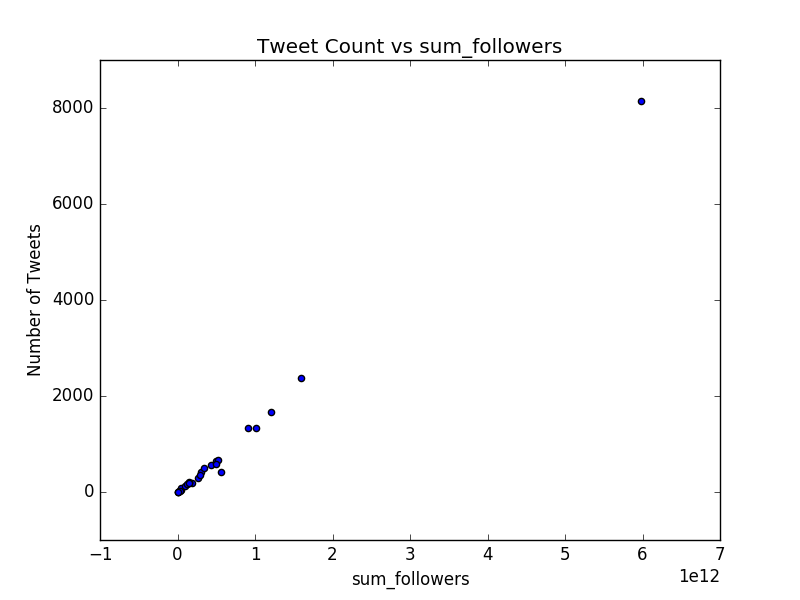
\includegraphics[width=\textwidth]{figures/count_vs_sum_tweets_superbowl.png}
\caption{Tweet Count vs Sum of Total Number of Followers}
\label{part1:fig:LC}
\end{subfigure}%
\hfill
\begin{subfigure}{.45\textwidth}
  \centering
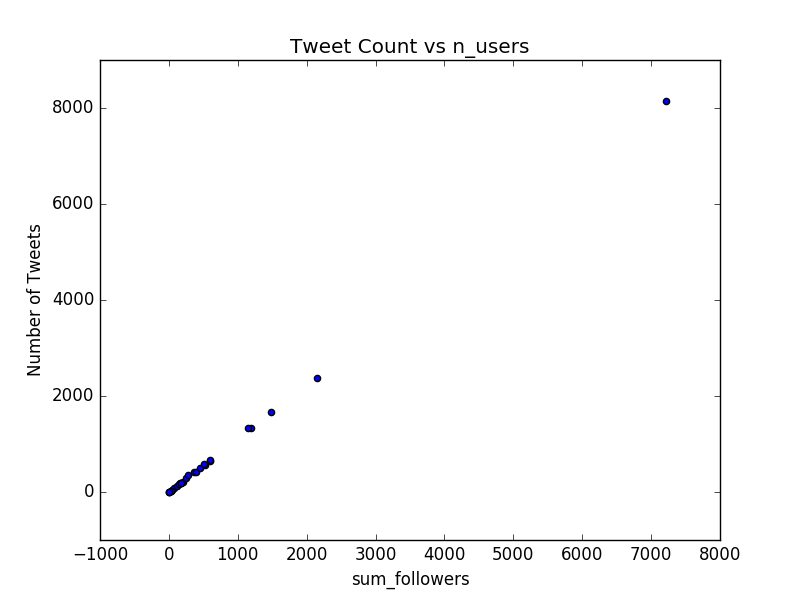
\includegraphics[width=\textwidth]{figures/count_vs_n_users_tweets_superbowl.png}
\caption{Tweet Count vs Number of Users Who Tweeted 3 or More Times Per Hour}
\label{part1:fig:LC}
\end{subfigure}

\begin{subfigure}{.45\textwidth}
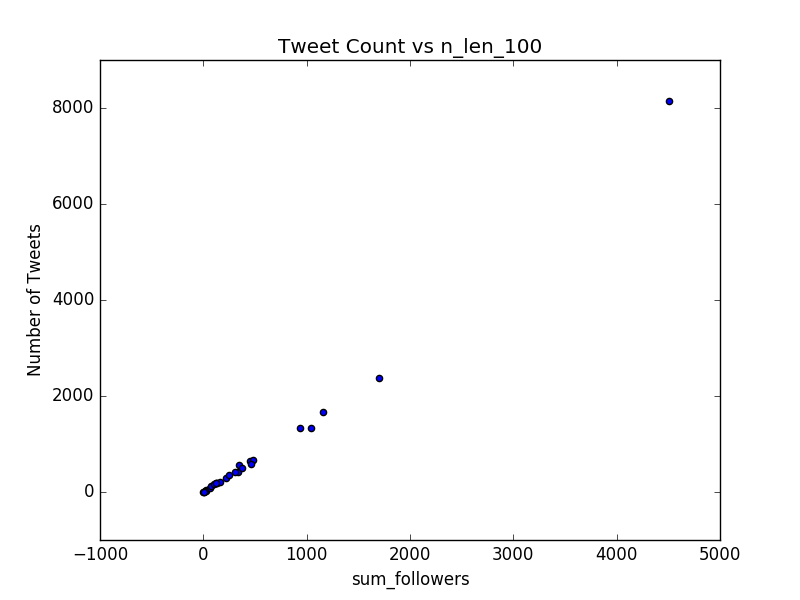
\includegraphics[width=\textwidth]{figures/count_vs_n_len_100_tweets_superbowl.png}
\caption{Tweet Count vs Number of Tweets with 100 or More Characters }
\label{part1:fig:LC}
\end{subfigure}

\caption{\#superbowl: Scatter plots for top 3 features in measurements}
\label{part1:fig}
\end{figure}

\subsection{Part 4:}

In part 4 we split our feature data into 10 parts for cross-validation. 10 tests are run and each time the model is fitted on 9 parts and the number of tweets is predicted for the 1 remaining part. The average prediction error is calculated over samples in the remaining part and then these values are averaged over the 10 tests.

Different regression models are then created according to the given three time periods (Period1: Before Feb 1, 8AM, Period 2: Between Feb 1, 8AM and Period 3: 8PM, and After Feb 1 8PM). These times reflect a period of time before the Super Bowl, the day including the actual Super Bowl game and a period of time after the Super Bowl. These periods of time are expected to follow respective trends of inactivity, then high bursting activity and then inactivity. Cross validation errors for the 3 models are reported in the tables below.


%gohawks
\begin{table}[H]
	\centering
	\begin{tabular}{| c | c | c | c |}
		\hline 
		Period & Average Prediction Error \\\hline
		1 & 27.448149 \\\hline
		2 & 36.383078 \\\hline 
		3 & 16.337346 \\\hline
	\end{tabular} 
	\caption{\#gohawks: Average prediction error for different periods (before, during, after)}
	\label{part1:tab1}
\end{table} 

%gopatriots
\begin{table}[H]
	\centering
	\begin{tabular}{| c | c | c | c |}
		\hline 
		Period & Average Prediction Error \\\hline
		1 & 61.608437 \\\hline
		2 & 65.836415 \\\hline 
		3 & 10.785898 \\\hline
	\end{tabular} 
	\caption{\#gopatriots: Average prediction error for different periods (before, during, after)}
	\label{part1:tab1}
\end{table} 

%nfl
\begin{table}[H]
	\centering
	\begin{tabular}{| c | c | c | c |}
		\hline 
		Period & Average Prediction Error \\\hline
		1 & 51.328586 \\\hline
		2 & 170.605770 \\\hline 
		3 & 27.154346 \\\hline
	\end{tabular} 
	\caption{\#nfl: Average prediction error for different periods (before, during, after)}
	\label{part1:tab1}
\end{table} 

%patriots
\begin{table}[H]
	\centering
	\begin{tabular}{| c | c | c | c |}
		\hline 
		Period & Average Prediction Error \\\hline
		1 & 84.086567 \\\hline
		2 & 65.676033 \\\hline 
		3 & 16.494728 \\\hline
	\end{tabular} 
	\caption{\#patriots: Average prediction error for different periods (before, during, after)}
	\label{part1:tab1}
\end{table} 

%sb49
\begin{table}[H]
	\centering
	\begin{tabular}{| c | c | c | c |}
		\hline 
		Period & Average Prediction Error \\\hline
		1 & 3436.743379 \\\hline
		2 & 1964.359263 \\\hline 
		3 & 40.565964 \\\hline
	\end{tabular} 
	\caption{\#sb49: Average prediction error for different periods (before, during, after)}
	\label{part1:tab1}
\end{table} 


%superbowl
\begin{table}[H]
	\centering
	\begin{tabular}{| c | c | c | c |}
		\hline 
		Period & Average Prediction Error \\\hline
		1 & 542.311391 \\\hline
		2 & 1533.897981 \\\hline 
		3 & 212.234838 \\\hline
	\end{tabular} 
	\caption{\#superbowl: Average prediction error for different periods (before, during, after)}
	\label{part1:tab1}
\end{table} 

\subsection{Part 5:}

The test data set was downloaded and our model was used to make predictions for the next hour in each test case. The predicted number of tweets for the next hour in each sample set are shown below.

%predicted
\begin{table}[H]
	\centering
	\begin{tabular}{| c | c | c | c |}
		\hline 
		Sample File & Predicted Tweets \\\hline
		1 & 60.125156 \\\hline
		2 & 99.887770 \\\hline 
		3 & 78000.896189 \\\hline
		4 & 603.955758 \\\hline
		5 & 276.738015 \\\hline
		6 & 287.107220 \\\hline
		7 & 41118.362584 \\\hline
		8 & 57.667595 \\\hline
		9 & 44.229527 \\\hline
		10 & 1551.637766 \\\hline
	\end{tabular} 
	\caption{Predicted number of tweets across sample files}
	\label{part1:tab1}
\end{table} 


\subsection{Part 6:}
In this portion we used bag of words representation of all the tweets regarding gopatriots and gohawks to formulate a sparse model to categorize future tweets based on the context of the tweets themselves. To start, we created a JSON parsing function to detect tweet bodies from the JSON structures. We then output each tweet into their own .txt file for sklearn to import and fit our model. For all .txt files related to gopatriots and gohawks we produced a sparse feature vector of words which excluded the words gopatriots and gohawks to discard any bias terms the sklearn?s Logistic Regression would be skewed upon. After using the TFIDF Vectorizer from the sklearn library, we were able to create a numerical representation of our tweets. As mentioned previously, we used the Logistic Regression algorithm in a 10-fold cross-validation accuracy calculation. We observed the following results of classifying tweets between gopatriots and gohawks.

%CrossValidation Scores
\begin{table}[H]
	\centering
	\begin{tabular}{| c | c | c | c |}
		\hline 
		Iteration & Cross Validation Score \\\hline
		1 & 91.11\% \\\hline
		2 & 91.70\% \\\hline 
		3 & 91.54\% \\\hline
		4 & 91.53\% \\\hline
		5 & 91.51\% \\\hline
		6 & 91.44\% \\\hline
		7 & 91.48\% \\\hline
		8 & 91.45\% \\\hline
		9 & 91.59\% \\\hline
		10 & 91.40\% \\\hline
		Mean Accuracy & 91.47\% \\\hline

	\end{tabular} 
	\caption{\: 10-Fold Cross Validation Scores}
	\label{part1:tab1}
\end{table} 


\end{document}